    \section{Pomiar napięcia}
         Pomiar napięcia dokonywany jest przy użyciu przetwornika analogowo-cyfrowego wbudowanego w mikroprocesor \cite{esp32}. Posiada on bowiem dwa 12 bitowe przetworniki, których wejścia są multipleksowane na aż 18 pinów. Po wczytaniu się w dokumentację okazuje się jednak że użyteczność tych przetworników ma wiele wykluczeń. Najważniejszym z nich jest interferencja przetwornika ADC2 z peryferium odpowiedzialnym za połączenie WiFi. Oznacza to że w projektach od których wymagamy stałego połączenia z siecią jesteśmy ograniczeni jedynie do 8 pinów obsługujących odczyty analogowe. 
         
         Kolejnym ciekawym aspektem tego układu jest możliwość programowego wyboru tłumienia sygnału wejściowego. Producent umożliwia nam wybór od 0dB poprzez 2.5dB oraz 6dB aż do 11dB tłumienia. Im wyższy parametr zostanie wybrany tym wyższe napięcia jest w stanie obsłużyć przetwornik. Niemniej jednak wybór wyższych oczek znacznie degraduje precyzję pomiaru.
     
     
    \subsection{Konfiguracja ADC}
        Po dokładnym przestudiowaniu dokumentacji przyjęte zostało ustawienie tłumienia na poziomie 2,5dB. Patrz \ref{code:adc1}. Wyższe ustawienia wprowadzają znaczną niedokładność pomiarów. Według dokumentacji \cite{esp32} takie ustawienie sprawia że efektywny zakres pomiarowy kształtuje się w zakresie od 100mV do 1250mV na pinie mikrokontrolera. Błędy pomiaru zadeklarowane przez producenta nie powinny przekroczyć $ \pm 30 mV$. Jednakże, zasilanie płytki jest zaprojektowane do obsługi dużo większych napięć, tak aby móc wykorzystywać szeroki zakres silników. Podanie napięcia wyższego jak zasilanie procesora, które w tym wypadku wynosi 3.3V, spowodowałoby trwałe uszkodzenia układu. Do bezpiecznego pomiaru napięcia zasilania niezbędne jest więc zastosowanie dzielnika napięcia. 
        
        Rozdzielczość peryferium została ustawiona na 12 bitów. Wynika z tego że istnieje $2^{12} = 4096$ poziomów kwantyzacji. Nie spodziewam się że mój autorski projekt płytki drukowanej \ref{fig:pcb} będzie miał na tyle niski szum kwantyzacji, aby móc w pełni wykorzystać taką rozdzielczość, ale w tym przypadku czas pomiaru nie jest tutaj kluczowy. Założenie wykonywania pomiaru zakłada że i tak będzie wykonywane wiele pomiarów pod rząd, aby później móc wyciągnąć z nich średnią.
        
        \begin{kod}
          \inputminted[firstline=8,lastline=17]{cpp}{esp/listings/adc.cpp}
          \caption{Konfiguracja przetwornika ADC}
          \label{code:adc1}
          \vspace{2em}
        \end{kod}
        

    

        
    \subsection{Dzielnik napięcia}
        Zadecydowałem że w tym projekcie wystarczający będzie najprostszy dzielnik oparty na dwóch rezystorach. Pozwoli nam on liniowo podzielić napięcie, tak aby nigdy nie przekroczyło ono wartości niebezpiecznej dla mikroprocesora. Do stworzenia dzielnika wykorzystałem rezystory z szeregu E24 \cite{szereg} o wartościach $9.1k \Omega $ oraz $1k \Omega $ i podłączyłem je w sposób pokazany na schemacie \ref{fig:pcb_schematic_1}.
        
        Obliczenie dostępnego zakresu pomiarowego przetwornika adc odbywa się przy pomocy wzoru na dzielnik napięcia \cite{dzielnik}. Jest on następujący:
        
        \vspace{1em}
        \begin{displaymath}
          V_{out} = \frac{ R_2 }{ R_1 + R_2 } \cdot V_{in}
        \end{displaymath}
        \vspace{1em}
        
        Gdzie napięcie wejściowe $V_{out}$ jest maksymalnym napięciem dostępnym na wejściu przetwornika. Zgodnie z informacją zawartą w dokumentacji procesora \cite{esp32} wybranie tłumienia na poziomie 2.5dB skutkuje otrzymaniem 1250mV jako granicy efektywnego zakresu pomiarowego. Przy czym producent zaznacza że ta wartość zależy od konkretnego egzemplarza i może się wahać. $R_1$ oraz $R_2$ to użyte rezystory w dzielniku. W tym przypadku są to kolejno $9.1k \Omega $ oraz $1k \Omega $.
        
        Dla maksymalnego obsługiwanego napięcia z przedziału wzór to:
        
        \vspace{1em}
        \begin{displaymath}
          1.250V = \frac{ 1k \Omega  }{ 9.1k \Omega  + 1k \Omega  } \cdot V_{in}
        \end{displaymath}
        \vspace{1em}
        
        Po przekształceniu go tak aby wyliczyć napięcie przed dzielnikiem otrzymujemy:
        
        \vspace{1em}
        \begin{displaymath}
         V_{in} = \frac{ 1.250V \cdot (9.1k \Omega  + 1k \Omega)  }{ 1k \Omega  } = 12.625 V
        \end{displaymath}
        \vspace{1em}
        
        Dla najniższego napięcia w mieszczącego się w zakresie efektywnego pomiaru (100mV) otrzymamy:
        
        \vspace{1em}
        \begin{displaymath}
         V_{in} = \frac{ 0.100V \cdot (9.1k \Omega  + 1k \Omega)  }{ 1k \Omega  } = 1.01 V
        \end{displaymath}      
        \vspace{1em}
        
        Oznacza to że w zakresie zasilania od $1.01V$ do $12.625V$ mamy dużą szansę uzyskać wynik pomiaru bliski rzeczywistemu.
        
    \newpage
        
    \subsection{Wyznaczanie współczynnika konwersji}
        W celu przeliczenia wartości odczytywanych z przetwornika analogowy-cyfrowego na napięcie wyrażone w woltach, niezbędne jest wyznaczenie współczynnika konwersji. 
        
        Posiadając wiedzę na temat użytych rezystorów w dzielniku napięcia, jest możliwe wyliczenie tego współczynnika. Aczkolwiek, moje doświadczenie z projektowaniem układów pomiarowych podpowiada że teoria bardzo często mija się z praktyką i zazwyczaj kalibruję swoje układy wykonując serię pomiarów. Tak też zrobiłem w tym przypadku. Wyniki zostały przedstawione na wykresie \ref{fig:adc_plot}
 
        \begin{figure}
        \vspace{1em}
            \centering
            \begin{tikzpicture}
                \centering
                \begin{axis}[ylabel = adc readings, xlabel = voltage, legend pos=north west, ymajorgrids=true, grid style=dashed, width=0.9\textwidth]
                    \addplot table [x=a, y=b, col sep=comma] {esp/adc_plot.dat};
                    \addlegendentry{\(ADC_{RAW}\)}
                    \addplot [domain=4.8:14.5, samples=100, color=red] {x*308 - 292};
                    \addlegendentry{\(x*308 - 292\)}
                \end{axis}
            \end{tikzpicture}
            \caption{Pomiary danych ADC do napięcia zasilania}
            \label{fig:adc_plot}
        \end{figure}
        \vspace{1em}
        
        %TODO dodać opis osi, jednostki, czerwoną linię regresji  
        
        Uzyskane pomiary potwierdzają że prawie cały zakres przetwornika, nie licząc końców, jest liniowy. Pomiary zakończyłem przy około $5.1V$ ponieważ poniżej tej wartości stabilizator liniowy, użyty do obniżenia napięcia na procesorze, przestawał poprawnie działać, co kończyło się resetami jednostki centralnej.
        
        Dzięki regresji liniowej byłem w stanie wyprowadzić równanie, które w łatwy sposób umożliwia przeliczanie odczytów z ADC na wartość napięcia.
        
        \vspace{1em}
        \begin{displaymath}
          y = \frac{ ADC_{RAW} + 292 }{ 398 }
        \end{displaymath}    
        \vspace{1em}
        
        Za $ADC_{RAW}$ wstawiamy wartość pomiaru i otrzymujemy napięcie wyrażone w woltach.
        
        
        
        
    \subsection{Rozdzielczość pomiaru}
        Posiadając już możliwość przeliczania surowych odczytów na napięcie, należałoby wyznaczyć rozdzielczość otrzymanych danych. Do obliczenia rozdzielczości napięciowej, czyli najmniejszego możliwego skoku zdolnego do zapisania przed przetwornik, musimy wykonać dwa pomiary. Następnie należy porównać różnice obliczonych napięć do różnicy surowych danych. Przy pomocy podanego wzoru:
        
        \vspace{1em}
        \begin{displaymath}
          \frac{ V_{1} - V_{2} }{ ADC_{1} - ADC_{2} } = \frac{ 10.136V - 6.171V  }{ 2826 - 1609 } = \frac{ 3.965V }{ 1217 } = 0.0032V
        \end{displaymath}    
        \vspace{1em}
          
          
    \subsection{Wykonywanie pomiarów}
        Wykonywanie pomiarów jest wykonywane na osobnym procesie. Dzięki temu można w łatwy sposób kontrolować częstotliwość mierzenia napięcia i wysyłania danych z ADC na MQTT. Pętla wyzwalająca odczyt wykonuje się raz na 20 milisekund. W każdej iteracji następuje pomiar, a odczytana wartość umieszczana jest w buforze. Co dziesiąta iteracja wylicza średnią z pomiarów, konwertuje wartość na wolty i wysyła dany na MQTT. Diagram aktywności umieszczony został w listingu \ref{fig:adc_plantuml}. 
        
 
        
        \begin{kod}
          \inputminted[firstline=19, lastline=44]{cpp}{esp/listings/adc.cpp}
          \caption{Wyzwalanie pomiaru i przeliczanie wartości}
          \label{code:adc2}
          \vspace{2em}
        \end{kod}
        
        
        \begin{figure}[ht]
          \centering
          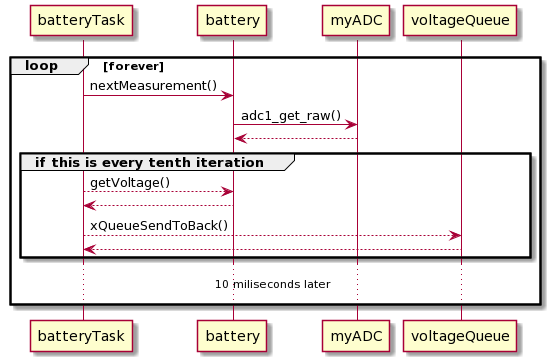
\includegraphics[width=0.8\textwidth]{img/adc_uml.png}
          \caption{Diagram aktywności dokonywania pomiarów}
          \label{fig:adc_plantuml}
        \end{figure}
 
        
        
        
        
        % 1000 i 9100
        % 1021 i 9273
        % y = 308*x -292
        % x = y+292 / 308
        
        
        